\documentclass[../main.tex]{subfile}

\begin{document}

\tikzset{/tkzmkangle/mark=none}

\topictitle{Argand Diagrams}

\sectitle{The Diagram}

An Argand diagram is a way of representing complex numbers on a 2D plane. The horizontal axis is the real numbers, and the vertical axis is the imaginary numbers.

\begin{figure}[H]
	\begin{minipage}{0.65\linewidth}
	\begin{center}
	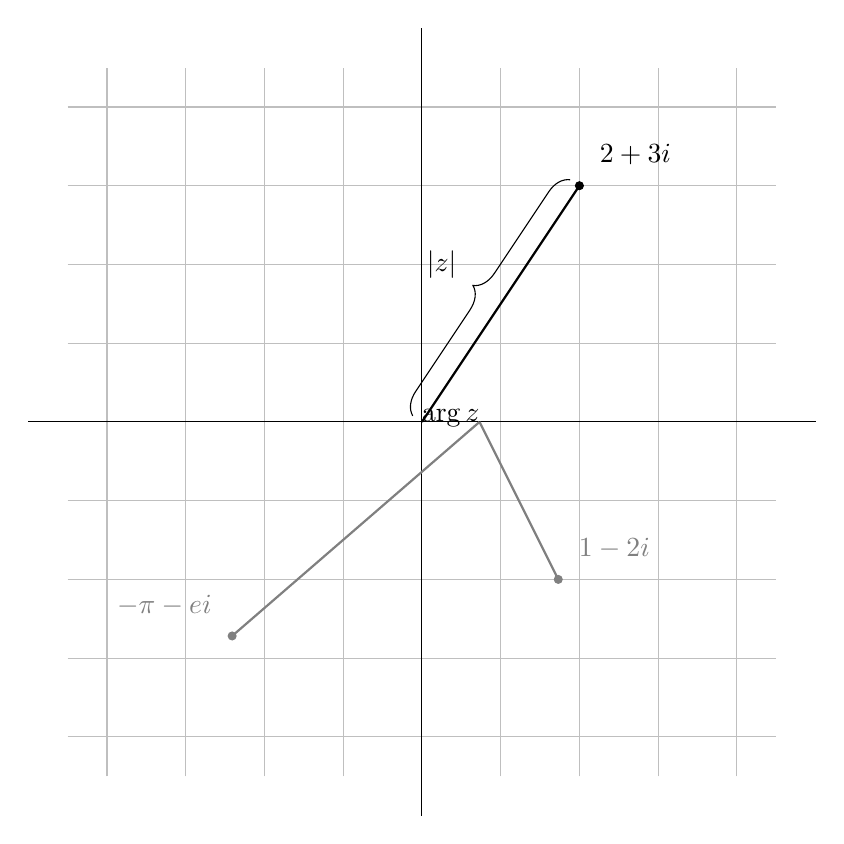
\begin{tikzpicture}
		\coordinate (O) at (0,0);

		\draw[step=1, lightgray, thin] (-4.5,-4.5) grid (4.5,4.5);
		\draw (-5,0) -> (5,0);
		\draw (0,-5) -> (0,5);

		\draw[thick] (0,0) -- (2,3);
		\draw[fill=black] (2,3) circle[radius=0.05];
		\node[label={[label distance=0.5]45:$2 + 3i$}] (2,3) at (2,3) {};

		\draw[decorate, decoration={brace, amplitude=8pt, raise=4pt}] (0,0) -- node[above, xshift=-0.75cm, yshift=0.2cm] {$|z|$} (2,3);

		\coordinate (A) at (2,3);
		\coordinate (B) at (1,0);
		\tkzMarkAngle[size=0.75](B,O,A);
		\tkzLabelAngle[pos=1.2](B,O,A){$\arg z$};

		\begin{scope}[
			every node/.style={gray},
			every path/.style={gray},
		]
			\draw[thick] (0,0) -- (1,-2);
			\draw[fill=gray] (1,-2) circle[radius=0.05];
			\node[label={[label distance=0.5]45:$1 - 2i$}] (1,-2) at (1,-2) {};

			\draw[thick] (0,0) -- (-3.14159,-2.7182818);
			\draw[fill=gray] (-3.14159,-2.7182818) circle[radius=0.05];
			\node[label={[label distance=0.5]135:$-\pi - ei$}] (-pi,-e) at (-3.14159,-2.7182818) {};
		\end{scope}
	\end{tikzpicture}
	\end{center}
	\end{minipage}\hfill
	\begin{minipage}{0.33\linewidth}
		\setlength{\parskip}{1em}
		The modulus $|z|$ of a complex number $z$ is the distance from the point to the origin. The argument $\arg z$ is the angle between the vector line and the positive real axis.

		For a modulus $|z| = r$ and an argument $\arg z = \theta$, the modulus-argument form of $z$ is $\boxed{r(\cos\theta + i \sin\theta)}$.

		Multiplication is unaffected by the modulus, so $|zw| = |z||w|$ and $\left|\dfrac{z}{w}\right| = \dfrac{|z|}{|w|}$.

		Multiplication is additive over $\arg$, so $\arg(zw) = \arg z + \arg w$ and $\arg\left(\dfrac{z}{w}\right) = \arg z - \arg w$.

		$|z - w|$ is the distance between $z$ and $w$.
	\end{minipage}
\end{figure}

\sectitle{Loci}

\begin{figure}[H]
	\begin{minipage}{0.65\linewidth}
	\begin{center}
	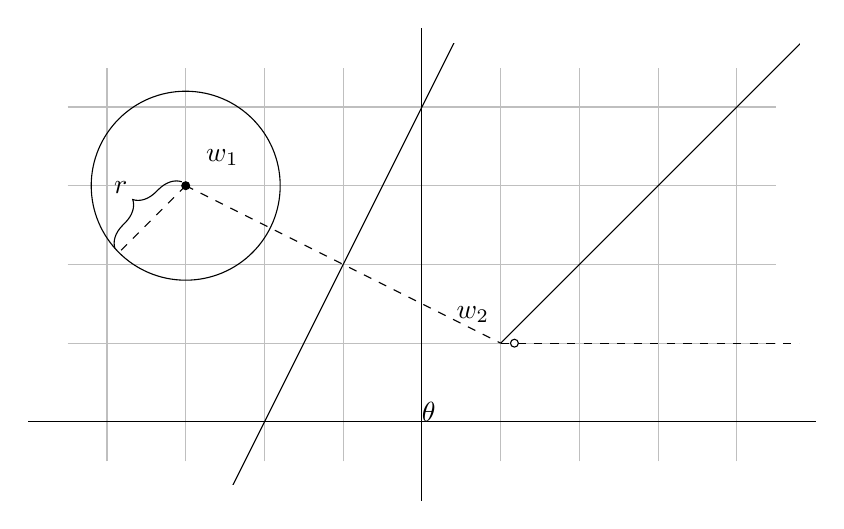
\begin{tikzpicture}
		\coordinate (O) at (0,0);

		\draw[step=1, lightgray, thin] (-4.5,-0.5) grid (4.5,4.5);
		\draw (-5,0) -> (5,0);
		\draw (0,-1) -> (0,5);

		\coordinate (circle center) at (-3,3);
		\draw[fill=black] (circle center) circle[radius=0.05];
		\node[label={[label distance=0.5]45:$w_1$}] (w1) at (circle center) {};
		\draw (circle center) circle[radius=1.2];

		\draw[dashed] (circle center) -- ++(225:1.2);
		\draw[decorate, decoration={brace, amplitude=8pt, mirror, raise=2pt}] (circle center) -- node[above, xshift=-0.4cm, yshift=0.2cm] {$r$} ++(225:1.2);

		\coordinate (other point) at (1,1);
		\node[label={[label distance=0.5]100:$w_2$}] (w2) at (other point) {};

		\draw[dashed] (circle center) -- (other point);

		\begin{scope}
			\clip (-4.8,-0.8) rectangle (4.8,4.8);
			\draw (1,6) -- (-5,-6);
			\draw[dashed] (other point) -- (5,1);
			\draw (other point) -- ++(45:10);
		\end{scope}

		\coordinate (A) at (2,1);
		\coordinate (B) at (3,3);
		\tkzMarkAngle[size=0.8](A,other point,B);
		\tkzLabelAngle[pos=0.95](A,other point,B){$\theta$};

		\draw[fill=white] (other point) circle[radius=0.05];
	\end{tikzpicture}
	\end{center}
	\end{minipage}\hfill
	\begin{minipage}{0.33\linewidth}
		\setlength{\parskip}{1em}
		For a complex number $w_1 = x + yi$, the locus of points $|z - w_1| = r$ \textcolor{gray}{$\Leftrightarrow \left|z - (x + yi)\right| = r$} is a circle of radius $r$ around the point $w$.

		$|z - w_1| = |z - w_2|$ is the perpendicular bisector of the line joining $w_1$ and $w_2$.

		$\arg(z - w_2) = \theta$ is a half-line from, but not including, the point $w$ making an angle $\theta$ from the real axis.
	\end{minipage}
\end{figure}

\end{document}
